\chapter{Inverse Trigonometric Functions}

Recall from the chapter on Functions that an inverse of a function is a machine that turns $y$ back into $x$. The inverses of trigonometric functions are essential to solving certain integrals (you will learn in a future chapter why integrals are useful - for now, trust us that they are!). Let's begin by discussing the $\sin$ function and its inverse, $\sin^{-1}$, also called $\arcsin$. 

\begin{figure}
\centering
	\begin{tikzpicture}
		\begin{axis}
		[axis lines = center, 
		xlabel=$x$,
		xmin=-3.142, 
		xmax=6.283, 
		xtick={-3.142, -1.571, 0, 1.571, 3.142, 4.712, 6.283}, 
		xticklabels={$-\pi$, $\frac{-\pi}{2}$, $0$, 
		$\frac{\pi}{2}$, $\pi$, $\frac{3\pi}{2}$, $2\pi$}, 
		ylabel=$y$,
		ymin = -1.25, 
		ymax=1.25, 
		ytick={-1, 1}]
		\addplot[blue, thick, samples=100]{sin(deg(x))};
		\addplot[red, dashed]{0.667};
		\end{axis}
	\end{tikzpicture}
	\caption{The horizontal line $y=\frac{2}{3}$ crosses $y = \sin{x}$ more than once}
	\label{fig:sinhline}
\end{figure}

Examine the graph of $\sin{x}$ in figure \ref{fig:sinhline}. See how the dashed horizontal line crosses the function at many points? This means the function $\sin{x}$ is not one-to-one. That is: there is not a unique $x$-value for every $y$-value. This means that if we do not restrict the domain of $\arcsin{x}$, the result will not be a function (see figure \ref{fig:arcsinvline}). In figure \ref{fig:arcsinvline}, you can see that just reflecting the graph across $y=x$ fails the vertical line test: an $x$ value has more than one $y$ value.

\begin{figure}
	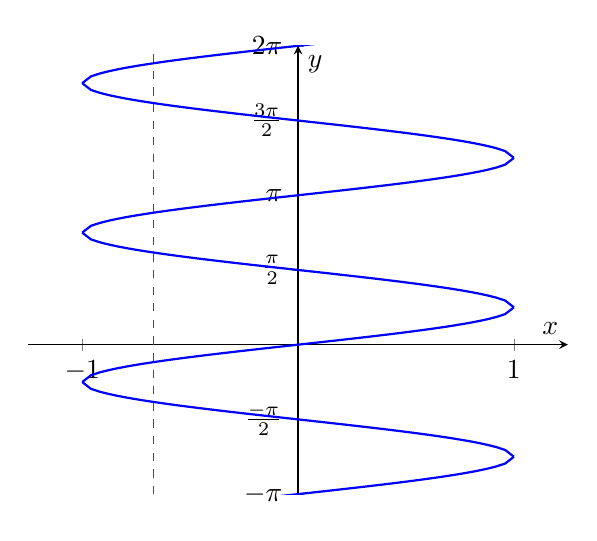
\begin{tikzpicture}
		\begin{axis}
		[axis lines = center, 
		xlabel=$x$,
		ymin=-360,
		ymax=720, 
		ytick={-360, -180, 0, 180, 360, 540, 720}, 
		yticklabels={$-\pi$, $\frac{-\pi}{2}$, $0$, 
		$\frac{\pi}{2}$, $\pi$, $\frac{3\pi}{2}$, $2\pi$}, 
		ylabel=$y$,
		xmin = -1.25, 
		xmax=1.25, 
		xtick={-1, 1}]
		\addplot[blue, thick, samples=50, domain=-1:1]{asin(x)};
		\addplot[blue, thick, samples=50, domain=-1:1]{asin(x)-360};
		\addplot[blue, thick, samples=50, domain=-1:1]{-asin(x)-180};
		\addplot[blue, thick, samples=50, domain=-1:1]{-asin(x)+180};
		\addplot[blue, thick, samples=50, domain=-1:1]{asin(x)+360};
		\addplot[blue, thick, samples=50, domain=-1:1]{-asin(x)+540};
		\addplot[blue, thick, samples=50, domain=-1:1]{asin(x)+720};
		\addplot[red, dashed]coordinates{(-0.67, -360) (-0.67, 720)};
		\end{axis}
	\end{tikzpicture}
	\caption{The inverse of an unrestricted $\sin$ function fails the vertical line test}
	\label{fig:arcsinvline}
\end{figure} 

\section{Derivatives of Inverse Trigonometric Functions}

\begin{center}
\begin{tabular}{ |c|c| }
	\hline
	$f$ & $f'$\\
	\hline
	$\arcsin{x}$ & $\frac{1}{\sqrt{1 - x^2}}$\\
	\hline
	$\arccos{x}$ & $ - \frac{1}{\sqrt{1 - x^2}}$\\
	\hline
	$\arctan{x}$ & $\frac{1}{1 + x^2}$\\
	\hline
	arccsc $x$ & $ - \frac{1}{x\sqrt{x^2-1}}$\\
	\hline
	arcsec $x$ & $\frac{1}{x\sqrt{x^2-1}}$\\
	\hline
	arccot $x$ & $ - \frac{1}{1+x^2}$\\
	\hline
\end{tabular}
\end{center}


\section{Practice}

\begin{Exercise}[label=invtrig1]
Find the $f'$. Give your answer in a simplified form. 
\begin{enumerate}
\item $f(x) = \arctan{x}^2$
\item $f(x) = x\text{arcsec }(x^3)$
\item $f(x) = \arcsin{\frac{1}{x}}$
\end{enumerate}
\end{Exercise}

\begin{Answer}[ref=invtrig1]
\begin{enumerate}
\item By the chain rule, $f'(x) = 2\arctan{x} \times \frac{d}{dx}\arctan{x} = 2\arctan{x}\frac{1}{1 + x^2}$
\item By the Product rule, $f'(x) = x \frac{d}{dx}\text{arcsec }(x^3) + \text{arcsec }(x^3)$. Further, by the chain rule, $\frac{d}{dx}\text{arcsec }(x^3) = \frac{1}{(x^3)\sqrt{(x^3)^2-1}} \times \frac{d}{dx}(x^3) = \frac{3x^2}{x^3\sqrt{x^6-1}}$. Therefore, $f'(x) = \frac{3}{\sqrt{x^6-1}} + \text{arcsec }(x^3)$
\item By the chain rule, $f'(x) = \frac{1/x}{\sqrt{1-(1/x)^2}} \times - \frac{1}{x^2} = - \frac{1}{x^3\sqrt{1-\frac{1}{x^2}}}$
\end{enumerate}
\end{Answer}